\documentclass[a4paper, 11pt]{article} % A4 paper size and default 11pt font size

\usepackage[margin=1.1in]{geometry}% http://ctan.org/pkg/geometry
\usepackage[utf8]{inputenc} % Required for inputting international characters
\usepackage[T1]{fontenc} 	% Output font encoding for international characters
\usepackage{stix} 			% Use the STIX fonts
\usepackage{parskip}        % I don't want indentation
\usepackage{yfonts} 		% More fonts
\usepackage{allrunes}		% Runes for the Title page
\usepackage{tcolorbox}		% Adds Colored boxes
\usepackage{enumitem}		% Make Listes
\usepackage{multirow}		% Fancyer tables
\usepackage{epigraph}		% Chapter quotes
\usepackage{framed}			% Quotes
\usepackage[strict]{changepage}
\usepackage{hyperref}		% Internal referances
\usepackage{booktabs}		% Booklist and referances
\usepackage{longtable}		% Multi page tables
\usepackage{tikz}			% Vertical Rune Text
	\usetikzlibrary{calc}
\usepackage{color, colortbl}% Custome colors
	\definecolor{Gray}{gray}{0.9}
	\definecolor{CadetBlue}{rgb}{0.37,0.62,0.63}
	\definecolor{LightCyan}{rgb}{0.88,1,1}
\usepackage{graphicx}		% Grafics and pictures
	\graphicspath{{./images/}}
\usepackage{censor} 		% Used to make redacted copy

\newcommand\blankpage{		% Add a blank page that dosen't count to total page numbers
    \clearpage \null
    \thispagestyle{empty}
    \addtocounter{page}{-1}
    \clearpage
}

\usepackage{censor} 		% Used to make redacted copy
\usepackage{cite}
\usepackage[title]{appendix}
\usepackage{titlesec}

%Quotations
\setlength\epigraphwidth{12cm}
\setlength\epigraphrule{0pt}

% environment derived from framed.sty: see leftbar environment definition
\definecolor{FormalShade}{rgb}{0.95,0.95,1}
\definecolor{DarkBlue}{rgb}{0.0, 0.0, 0.55}

\newenvironment{formal}{%
  \def\FrameCommand{%
    \hspace{1pt}%
    {\color{DarkBlue}\vrule width 2pt}%
    {\color{FormalShade}\vrule width 4pt}%
    \colorbox{FormalShade}%
  }%
  \MakeFramed{\advance\hsize-\width\FrameRestore}%
  \noindent\hspace{-4.55pt}% disable indenting first paragraph
  \begin{adjustwidth}{}{7pt}%
  \vspace{2pt}\vspace{2pt}%
}
{%
  \vspace{2pt}\end{adjustwidth}\endMakeFramed%
}


\newcounter{cnt} \setcounter{cnt}{0}

%Helper function to set counters
\def\inc{\stepcounter{cnt}\thecnt}

%Helper fuction to set margines
\def\changemargin#1#2{\list{}{\rightmargin#2\leftmargin#1}\item[]}
  \let\endchangemargin=\endlist 

%Lists boxes
\usepackage{amssymb}% http://ctan.org/pkg/amssymb
\usepackage{pifont}% http://ctan.org/pkg/pifont
\newlist{todolist}{itemize}{2}
\setlist[todolist]{label=$\square$}
\newcommand{\cmark}{\ding{51}}%
\newcommand{\xmark}{\ding{55}}%
\newcommand{\correct}{\rlap{$\square$}{\raisebox{0.5pt}{\large\hspace{1pt}\cmark}}%
\hspace{-2.5pt}}
\newcommand{\incorrect}{\rlap{$\square$}{\large\hspace{1pt}\xmark}}

\begin{document}
\StopCensoring %Add this line to create a non-Redacted version

%----------------------------------------------------------------------------------------
%	TITLE PAGE
%----------------------------------------------------------------------------------------
\begin{titlepage}
\begin{changemargin}{-1cm}{-1cm} 

\begin{minipage}[t]{500px}
	\vspace{-60px}
	\raggedleft 
	
\includegraphics[width=0.18\linewidth]{Kvasir.png} \\				
	
\includegraphics[width=0.18\linewidth]{Logo.png} \\
	\textswab{Think evil, do good}~~ \\
\end{minipage}	
\begin{minipage}[l][10px]{20px}	
	\tikz[remember picture, overlay]
    \node [rotate=90.2] at ($(current page.center)+(-9,0)$) 
    {
	\Large
	\underline{
\textarc{hinkewildogoodthinkewildogoodthinkewildogoodthinkewildogoodthinkewildogoodthinkewildogoodthinkewildogoodthinkewildogoodthinkewildogoodthinkewildogood} 
	}	
	};
\end{minipage}

\begin{minipage}[c]{490px}
\begin{changemargin}{5px}{5px}
	\center
	\Huge 
	\textbf{MS Azure Security Technologies} %Overskrift 
	\\
 	\vspace{3px}
	\Large
	AZ-500 Certification \\ %Underoverskrift
	\small 
	\censor{The Collective Conspiracy Coven of Conspicuous Insight and Contagious Brilliance}	%Tagline
\end{changemargin}
\end{minipage}

\vspace{480px}
\center
Version 1.0\\ %Version
\censor{\today} %Dato
\end{changemargin}
\end{titlepage}

%----------------------------------------------------------------------------------------

% Table Of Content  %
\pagenumbering{gobble}
\tableofcontents

% Content  %
\pagenumbering{arabic}
\setcounter{page}{1}
\section{The Certification}
\subsection{The Candidates}
Candidates for this exam are Microsoft Azure security engineers who implement security controls, maintain the security posture, manages identity and access, and protects data, applications, and networks. Candidates identify and remediate vulnerabilities by using a variety of security tools, implements threat protection, and responds to security incident escalations. As a Microsoft Azure security engineer, candidates often serve as part of a larger team dedicated to cloud-based management and security and may also secure hybrid environments as part of an end-to-end infrastructure.

Candidates for this exam should have strong skills in scripting and automation, a deep understanding of networking, virtualization, and cloud N-tier architecture, and a strong familiarity with cloud capabilities, Microsoft Azure products and services, and other Microsoft products and services.

\subsection{Content Overview}
\begin{itemize}
\item Manage identity and access (20-25\%)
	\begin{itemize}
	\item Configure Microsoft Azure Active Directory for workloads
	\item Configure Microsoft Azure AD Privileged Identity Management
	\item Configure Microsoft Azure tenant security
	\end{itemize}
\item Implement platform protection (35-40\%)
	\begin{itemize}
	\item Implement network security
	\item Implement host security
	\item Configure container security
	\item Implement Microsoft Azure Resource management security
	\end{itemize}
\item Manage security operations (15-20\%)
	\begin{itemize}
	\item Configure security services
	\item Configure security policies
	\item Manage security alerts
	\end{itemize}
\item Secure data and applications (30-35\%)
	\begin{itemize}
	\item Configure security policies to manage data
	\item Configure security for data infrastructure
	\item Configure encryption for data at rest
	\item Implement security for application delivery
	\item Configure application security
	\item Configure and manage Key Vault
	\end{itemize}
\end{itemize}

\clearpage
\subsection{Prerequisites}
The AZ-500 Azure Security Engineer Exam, like the MS-500 exam, covers a wide range of topics and technologies. Before considering taking this exam, you should first have good knowledge in the Azure technologies themselves which makes sense. You should learn what are the different Azure platform technologies in order to learn how to secure them.

So a good way to do that is to take the Azure AZ-900 (Azure Fundamentals) or the AZ-103 (Azure Administrator) exam first to learn more about Azure technologies. Now this is not a requirement for taking the AZ-500 exam, but it is a good start. If you are familiar with Azure technologies, then you can go and take the AZ-500 Azure Security Engineer Exam right away.

\subsection{The exam}
The AZ-500 Azure Security Engineer Exam expects you to know how to implement security controls, maintain the security posture, manages identity and access, and protects data, applications, and networks.

As per the AZ-500 Azure Security Engineer Exam official documentation:
\begin{formal}
Candidates identify and remediate vulnerabilities by using a variety of security tools, implements threat protection, and responds to security incident escalations. As a Microsoft Azure security engineer, candidates often serve as part of a larger team dedicated to cloud-based management and security and may also secure hybrid environments as part of an end-to-end infrastructure
\end{formal}
\section{Certification Content}

\subsection{Manage identity and access (20-25\%)}

\subsubsection{Configure Microsoft Azure Active Directory for workloads}
\begin{itemize}
\item Create App registration \\
Tree Supported account types:
	\begin{itemize}
	\item Azure AD only single-tenant -> LOB app.
	\item Azure AD only multi-tenant -> All business and educational users.
	\item Azure AD multi-tenant and personal Microsoft accounts -> Widest set of users.
	\end{itemize}
\item Configure App registration permission scopes \\
Uses OAuth 2.0 for third parti app access.\\
MS strongly recommends that you use Microsoft Graph. \\
Two Permission types:
	\begin{itemize}
	\item Delegated permissions -> App permission $\cap$ User permission 
	\item Application permissions -> App permission  
	\end{itemize}
Interesting scopes: 
	\begin{itemize}
	\item openid -> Required for OpenID Connect.
	\item email -> access to the user's primary email address.
	\item profile -> access to a substantial amount of information about the user. See \href{https://docs.microsoft.com/en-us/azure/active-directory/develop/id-tokens}{id tokens}
	\item offline\_access -> Maintain access to data you have given it access to.
	\end{itemize}
\item Manage App registration permission consent \\
Consent can be given by individuals or by Admins for an entire tenant. \\
Admin consent can only be granted with the "admin consent endpoint"
\item Configure multi-factor authentication settings 
\item Manage Microsoft Azure AD directory groups 
\item Manage Microsoft Azure AD users 
\item Install and configure Microsoft Azure AD Connect 
\item Configure authentication methods 
\item Implement conditional access policies 
\item Configure Microsoft Azure AD identity protection 
\end{itemize}

\begin{tabular}{p{14cm} | r}
\textbf{Literature} & \\
\hline
\href{https://docs.microsoft.com/en-us/azure/active-directory/develop/quickstart-register-app}{Quickstart: Register an application with the Microsoft identity platform} & 3 \textcolor{gray}{(5)} \\
\href{https://docs.microsoft.com/en-us/azure/active-directory/develop/v1-permissions-and-consent}{Permissions and consent in the Azure Active Directory v1.0 endpoint} & 6 \\
\href{https://docs.microsoft.com/en-us/azure/active-directory/develop/v2-permissions-and-consent}{Permissions and consent in the Microsoft identity platform endpoint} & 18 \\
\href{https://docs.microsoft.com/en-us/azure/active-directory/authentication/howto-mfa-mfasettings}{Configure Azure Multi-Factor Authentication settings} & 21 \\
\href{https://docs.microsoft.com/en-us/microsoft-365/enterprise/identity-use-group-management}{Use groups for management} & 3 \\
\href{https://docs.microsoft.com/en-us/azure/active-directory/hybrid/how-to-connect-install-custom}{Custom installation of Azure AD Connect} & 26 \\
\href{https://docs.microsoft.com/en-us/azure/security/fundamentals/choose-ad-authn}{Authentication method for Azure Active Directory hybrid identity solution} & 15+13 \\
\href{https://docs.microsoft.com/en-us/azure/active-directory/conditional-access/best-practices}{Best practices for Conditional Access in Azure Active Directory} & 6 \\
\href{https://docs.microsoft.com/en-us/azure/active-directory/identity-protection/overview-identity-protection}{What is Azure Active Directory Identity Protection?} & 3 \\
\cline{2-2} 
 & 114
\end{tabular}

\subsubsection{Configure Microsoft Azure AD Privileged Identity Management}
\begin{itemize}
\item monitor privileged access 
\item configure access reviews 
\item activate Privileged Identity Management 
\end{itemize}

\begin{tabular}{p{14cm} | r}
\textbf{Literature} & \\
\hline
\href{https://docs.microsoft.com/en-us/azure/active-directory/privileged-identity-management/pim-getting-started}{Start using Privileged Identity Management} & 3 \\
\href{https://docs.microsoft.com/en-us/azure/active-directory/privileged-identity-management/pim-deployment-plan}{Deploy Azure AD Privileged Identity Management (PIM)} & 26 \\
\href{https://docs.microsoft.com/en-us/azure/active-directory/governance/access-reviews-overview}{What are Azure AD access reviews?} & 6+12 \\
\cline{2-2} 
 & 47 \\
\end{tabular}

\subsubsection{Configure Microsoft Azure tenant security}
\begin{itemize}
\item transfer Microsoft Azure subscriptions between Microsoft Azure AD tenants 
\item manage API access to Microsoft Azure subscriptions and resources 
\end{itemize}

\begin{tabular}{p{14cm} | r}
\textbf{Literature} & \\
\hline
\href{https://docs.microsoft.com/en-us/azure/billing/billing-subscription-transfer}{Transfer billing ownership of an Azure subscription to another account} & 10 \\
\href{https://docs.microsoft.com/en-us/azure/api-management/api-management-howto-aad}{Authorize developer accounts by using Azure Active Directory in Azure API Management} & 4 \\
\href{https://docs.microsoft.com/en-us/azure/active-directory/develop/authentication-flows-app-scenarios}{Authentication flows and application scenarios} & 10 \\
\href{https://docs.microsoft.com/en-us/azure/active-directory/develop/active-directory-graph-api}{Azure Active Directory Graph API} & 4 \\
\cline{2-2} 
 & 28 \\
\end{tabular}

\clearpage
\subsection{Implement platform protection (35-40\%)}

\subsubsection{Implement network security}
\begin{itemize}
\item configure virtual network connectivity 
\item configure Network Security Groups (NSGs) 
\item create and configure Microsoft Azure firewall 
\item create and configure application security groups 
\item configure remote access management 
\item configure baseline 
\item configure resource firewall 
\end{itemize}

\begin{tabular}{p{14cm} | r}
\textbf{Literature} & \\
\hline
\href{https://docs.microsoft.com/en-us/azure/virtual-network/virtual-networks-overview}{What is Azure Virtual Network?} & 5 \\
\href{https://docs.microsoft.com/en-us/azure/virtual-network/manage-network-security-group}{Create, change, or delete a network security group} & 13 \\
\href{https://docs.microsoft.com/en-us/azure/firewall/tutorial-firewall-deploy-portal}{Tutorial: Deploy and configure Azure Firewall using the Azure portal} & 7 \\
\href{https://azure.microsoft.com/en-gb/blog/applicationsecuritygroups/}{Application Security Groups now generally available in all Azure regions} & 6 \\
\href{https://docs.microsoft.com/en-us/azure/security/fundamentals/management}{Security management in Azure} & 20 \\
\href{https://docs.microsoft.com/en-us/azure/security-center/security-center-network-recommendations}{Protect your network resources in Azure Security Center} & 9 \\
\href{https://docs.microsoft.com/en-us/azure/storage/common/storage-network-security}{Configure Azure Storage firewalls and virtual networks} & 17 \\
\href{https://docs.microsoft.com/en-us/azure/sql-database/sql-database-firewall-configure}{Azure SQL Database and Azure SQL Data Warehouse IP firewall rules} & 11 \\
\cline{2-2} 
 & 88 \\
\end{tabular}

\subsubsection{Implement host security}
\begin{itemize}
\item configure endpoint security within the VM 
\item configure VM security 
\item harden VMs in Microsoft Azure 
\item configure system updates for VMs in Microsoft Azure 
\item configure baseline 
\end{itemize}

\begin{tabular}{p{14cm} | r}
\textbf{Literature} & \\
\hline
\href{https://docs.microsoft.com/en-us/azure/security/fundamentals/antimalware}{Microsoft Antimalware for Azure Cloud Services and Virtual Machines} & 10 \\
\href{https://docs.microsoft.com/en-us/azure/security/fundamentals/iaas}{Security best practices for IaaS workloads in Azure} & 12 \\
\href{https://blogs.msdn.microsoft.com/mvpawardprogram/2018/01/09/just-in-time-access-azure-vms/}{Harden Your Azure Infrastructure Using Azure Security Center Just-In-Time VM Access} & 10 \\
\href{https://docs.microsoft.com/en-us/azure/automation/automation-tutorial-update-management}{Manage updates and patches for your Azure VMs} & 10 \\
\href{https://docs.microsoft.com/en-us/azure/security-center/security-center-features-retirement-july2019#menu_securityconfigurations}{Retirement of Security Center features (July 2019)} & 7 \\
\cline{2-2} 
 & 49 \\
\end{tabular}

\subsubsection{Configure container security}
\begin{itemize}
\item configure network 
\item configure authentication 
\item configure container isolation 
\item configure AKS security 
\item configure container registry 
\item configure container instance security 
\item implement vulnerability management 
\end{itemize}

\begin{tabular}{p{14cm} | r}
\textbf{Literature} & \\
\hline
\href{https://docs.microsoft.com/en-us/azure/virtual-network/container-networking-overview}{Azure Virtual Network capabilities} & 3 \\
\href{https://docs.microsoft.com/en-us/azure/aks/kubernetes-service-principal}{Service principals with Azure Kubernetes Service (AKS)} & 6 \\
\href{https://azure.microsoft.com/mediahandler/files/resourcefiles/container-security-in-microsoft-azure/Open\%20Container\%20Security\%20in\%20Microsoft\%20Azure.pdf}{Container Security in Microsoft Azure} & 45 \\
\href{https://docs.microsoft.com/en-us/azure/aks/concepts-security}{Security concepts for applications and clusters in Azure Kubernetes Service (AKS)} & 6 \\
\href{https://docs.microsoft.com/en-us/azure/container-instances/container-instances-image-security}{Security considerations for Azure Container Instances} & 9 \\
\cline{2-2} 
 & 69 \\
\end{tabular}

\subsubsection{Implement Microsoft Azure Resource management security}
\begin{itemize}
\item create Microsoft Azure resource locks 
\item manage resource group security 
\item configure Microsoft Azure policies 
\item configure custom RBAC roles 
\item configure subscription and resource permissions 
\end{itemize}

\begin{tabular}{p{14cm} | r}
\textbf{Literature} & \\
\hline
\href{https://docs.microsoft.com/en-us/azure/azure-resource-manager/resource-group-lock-resources}{Lock resources to prevent unexpected changes} & 6 \\
\href{https://docs.microsoft.com/en-us/azure/role-based-access-control/overview}{What is role-based access control (RBAC) for Azure resources?} & 7 \\
\href{https://docs.microsoft.com/en-us/azure/governance/policy/tutorials/create-and-manage}{Tutorial: Create and manage policies to enforce compliance} & 14 \\
\href{https://docs.microsoft.com/en-us/azure/role-based-access-control/custom-roles}{Custom roles for Azure resources} & 4 \\
\href{https://docs.microsoft.com/en-us/azure/role-based-access-control/role-assignments-portal}{Manage access to Azure resources using RBAC and the Azure portal} & 6 \\
\cline{2-2} 
 & 37 \\
\end{tabular}

\clearpage
\subsection{Manage security operations (15-20\%)}

\subsubsection{Configure security services}
\begin{itemize}
\item configure Microsoft Azure monitor 
\item configure Microsoft Azure log analytics 
\item configure diagnostic logging and log retention 
\item configure vulnerability scanning 
\end{itemize}

\begin{tabular}{p{14cm} | r}
\textbf{Literature} & \\
\hline
\href{https://docs.microsoft.com/en-us/azure/azure-monitor/azure-management}{Azure Management - Monitoring} & 3 \\
\href{https://docs.microsoft.com/en-us/azure/azure-monitor/platform/manage-access}{Manage access to log data and workspaces in Azure Monitor} & 10 \\
\href{https://docs.microsoft.com/en-us/azure/azure-monitor/platform/resource-logs-overview}{Azure Resource logs overview} & 2 \\
\href{https://docs.microsoft.com/en-us/azure/security-center/security-center-vulnerability-assessment-recommendations}{Vulnerability assessment in Azure Security Center} & 4 \\
\cline{2-2} 
 & 19 \\
\end{tabular}

\subsubsection{Configure security policies}
\begin{itemize}
\item configure centralized policy management by using Microsoft Azure Security Center 
\item configure Just in Time VM access by using Microsoft Azure Security Center 
\end{itemize}

\begin{tabular}{p{14cm} | r}
\textbf{Literature} & \\
\hline
\href{https://docs.microsoft.com/en-us/azure/security-center/tutorial-security-policy}{Working with security policies} & 9 \\
\href{https://docs.microsoft.com/en-us/azure/security-center/security-center-just-in-time}{Manage virtual machine access using just-in-time} & 11 \\
\cline{2-2} 
 & 20 \\
\end{tabular}

\subsubsection{Manage security alerts}
\begin{itemize}
\item create and customize alerts 
\item review and respond to alerts and recommendations 
\item configure a playbook for a security event by using Microsoft Azure Security Center 
\item investigate escalated security incidents 
\end{itemize}

\begin{tabular}{p{14cm} | r}
\textbf{Literature} & \\
\hline
\href{https://docs.microsoft.com/en-us/azure/security-center/security-center-managing-and-responding-alerts}{Manage and respond to security alerts in Azure Security Center} & 2 \\
\href{https://docs.microsoft.com/en-us/azure/security-center/security-center-recommendations}{Security recommendations in Azure Security Center} & 2 \\
\href{https://docs.microsoft.com/en-us/azure/security-center/security-center-playbooks}{Security Playbook in Azure Security Center (Preview)} & 3 \\
\href{https://docs.microsoft.com/en-us/azure/security-center/security-center-features-retirement-july2019#menu_investigate}{Security alerts investigation} & 5 \\
\cline{2-2} 
 & 12 \\
\end{tabular}

\clearpage
\subsection{Secure data and applications (30-35\%)}
\subsubsection{Configure security policies to manage data}
\begin{itemize}
\item configure data classification 
\item configure data retention 
\item configure data sovereignty 
\end{itemize}

\begin{tabular}{p{14cm} | r}
\textbf{Literature} & \\
\hline
\href{https://docs.microsoft.com/en-us/azure/information-protection/infoprotect-settings-tutorial}{Tutorial: Configure Azure Information Protection policy settings that work together} & 8 \\
\href{https://docs.microsoft.com/en-us/rest/api/storageservices/setting-a-storage-analytics-data-retention-policy}{Setting a Storage Analytics data retention policy} & 2 \\
\href{https://docs.microsoft.com/en-us/azure/kusto/management/retention-policy}{Retention policy} & 2 \\
\href{https://docs.microsoft.com/en-us/azure/governance/policy/samples/allowed-locations}{Sample - Allowed region locations} & 5 \\
\cline{2-2} 
 & 17 \\
\end{tabular}

\subsubsection{Configure security for data infrastructure}
\begin{itemize}
\item enable database authentication 
\item enable database auditing 
\item configure Microsoft Azure SQL Database threat detection 
\item configure access control for storage accounts 
\item configure key management for storage accounts 
\item create and manage Shared Access Signatures (SAS) 
\item configure security 
	\begin{itemize}
		\item HDInsights
		\item Cosmos DB
		\item Microsoft Azure Data Lake
	\end{itemize} 
\end{itemize}

\begin{tabular}{p{14cm} | r}
\textbf{Literature} & \\
\hline
\href{https://docs.microsoft.com/en-us/azure/sql-database/sql-database-aad-authentication}{Use Azure Active Directory Authentication for authentication with SQL} & 9 \\
\href{https://docs.microsoft.com/en-us/azure/sql-database/sql-database-auditing}{Get started with SQL database auditing} & 12 \\
\href{https://docs.microsoft.com/en-us/azure/sql-database/sql-database-threat-detection}{Azure SQL Database Advanced Threat Protection for single or pooled databases} & 2 \\
\href{https://docs.microsoft.com/en-us/azure/storage/common/storage-security-guide}{Azure Storage security guide} & 44 \\
\href{https://docs.microsoft.com/en-us/azure/storage/common/storage-encryption-keys-portal}{Configure customer-managed keys for Azure Storage encryption from the Azure portal} & 2 \\
\href{https://docs.microsoft.com/en-us/azure/storage/common/storage-sas-overview}{Grant limited access to Azure Storage resources using shared access signatures (SAS)} & 11 \\
\href{https://docs.microsoft.com/en-us/azure/hdinsight/domain-joined/apache-domain-joined-configure-using-azure-adds}{Enterprise Security Package configurations with Azure Active Directory Domain Services in HDInsight} & 7 \\
\href{https://docs.microsoft.com/en-us/azure/cosmos-db/database-security}{Security in Azure Cosmos DB - overview} & 7 \\
\href{https://docs.microsoft.com/en-us/azure/data-lake-store/data-lake-store-network-security}{Virtual network integration for Azure Data Lake Storage Gen1} & 6 \\
\cline{2-2} 
 & 100 \\
\end{tabular}

\subsubsection{Configure encryption for data at rest}
\begin{itemize}
\item implement Microsoft Azure SQL Database Always Encrypted
\item implement encryption 
	\begin{itemize}
		\item database
		\item Storage Service
		\item disk
		\item backup
	\end{itemize}
\end{itemize}

\begin{tabular}{p{14cm} | r}
\textbf{Literature} & \\
\hline
\href{https://docs.microsoft.com/en-us/azure/sql-database/sql-database-always-encrypted}{Always Encrypted: Protect sensitive data and store encryption keys in the Windows certificate store} & 12 \\
\href{https://docs.microsoft.com/en-us/sql/relational-databases/security/encryption/transparent-data-encryption?view=sql-server-2017}{Transparent Data Encryption (TDE)} & 11 \\
\href{https://docs.microsoft.com/en-us/azure/storage/common/storage-service-encryption}{Azure Storage encryption for data at rest} & 8 \\
\href{https://docs.microsoft.com/en-us/azure/security/fundamentals/azure-disk-encryption-vms-vmss}{Azure Disk Encryption for virtual machines and virtual machine scale sets} & 2 \\
\href{https://docs.microsoft.com/en-us/azure/backup/backup-azure-backup-faq#encryption}{Azure Backup - Frequently asked questions} & 8 \\
\cline{2-2} 
 & 41 \\
\end{tabular}

\subsubsection{Implement security for application delivery}
\begin{itemize}
\item implement security validations for application development 
\item configure synthetic security transactions 
\end{itemize}

\begin{tabular}{p{14cm} | r}
\textbf{Literature} & \\
\hline
\href{https://docs.microsoft.com/en-us/azure/security/security-paas-deployments}{Securing PaaS deployments} & 12 \\
\href{https://docs.microsoft.com/en-us/azure/azure-monitor/app/transaction-diagnostics
}{Unified cross-component transaction diagnostics} & 4 \\
\cline{2-2} 
 & 16 \\
\end{tabular}

\subsubsection{Configure application security}
\begin{itemize}
\item configure SSL/TLS certs 
\item configure Microsoft Azure services to protect web apps 
\item create an application security baseline 
\end{itemize}

\begin{tabular}{p{14cm} | r}
\textbf{Literature} & \\
\hline
\href{https://docs.microsoft.com/en-us/azure/app-service/app-service-web-tutorial-custom-ssl}{Tutorial: Upload and bind SSL certificates to Azure App Service} & 9 \\
\href{https://docs.microsoft.com/en-us/azure/application-gateway/create-web-app}{Configure App Service with Application Gateway} & 5 \\
\href{https://docs.microsoft.com/en-us/azure/security/fundamentals/paas-deployments}{Securing PaaS deployments} & 12 \\
\cline{2-2} 
 & 26 \\
\end{tabular}

\subsubsection{Configure and manage Key Vault}
\begin{itemize}
\item manage access to Key Vault 
\item manage permissions to secrets, certificates, and keys 
\item manage certificates 
\item manage secrets 
\item configure key rotation 
\end{itemize}

\begin{tabular}{p{14cm} | r}
\textbf{Literature} & \\
\hline
\href{https://docs.microsoft.com/en-us/azure/key-vault/key-vault-secure-your-key-vault}{Secure access to a key vault} & 13 \\
\href{https://docs.microsoft.com/en-us/azure/key-vault/about-keys-secrets-and-certificates}{About keys, secrets, and certificates} & 26 \\
\href{https://docs.microsoft.com/en-us/azure/key-vault/key-vault-key-rotation-log-monitoring
}{Set up Azure Key Vault with key rotation and auditing} & 14 \\
\cline{2-2} 
 & 53 \\
\end{tabular}

\newpage
\bibliography{ref}
\bibliographystyle{IEEEtran}

\pagenumbering{roman}
\setcounter{page}{1}
\begin{appendices}
\section{Glossary}
\subsection{Acronyms}
\begin{description}
	\item[LOB] Line-of-business (application)
	\item[OIDC] OpenID Connect
	\item[SIEM] Security information and event management
	\item[MCAS] Microsoft Cloud App Security
\end{description}


\section{Extended notes}

%%% Notes for Manage identiy and access %%%
\subsection{Manage identity and access}

% Configure Microsoft Azure Active Directory for workloads
% This section contains notes on "Configure Microsoft Azure Active Directory for workloads" relevant subjects %
\subsubsection{Application management}
\begin{figure}[!h]
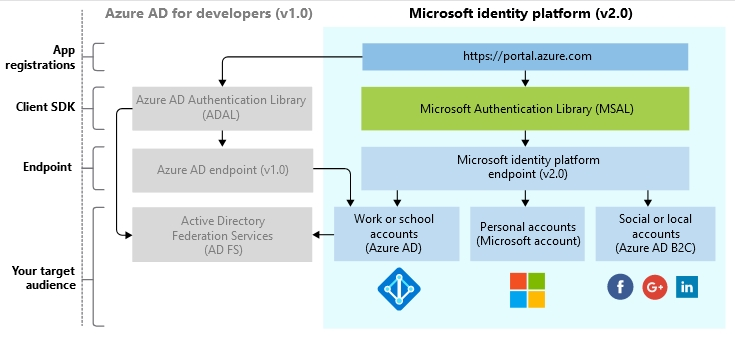
\includegraphics[width=1\textwidth]{microsoft-identity-platform.jpg}
\caption{Microsoft identity platform}
\end{figure}

\textbf{Permission / scope} \\
Azure AD defines two kinds of permissions:
\begin{itemize}
\item Delegated. Applications with signed in users. Can be either user or admin consent. The application is granted permission to act as the singed-in user when making requests. \\ Effective permissions are the \textit{least} privileged intersection of the delegated permissions for the application itself (through consent) and the privileges of the signed-in user. Within organizations, the privileges of the signed-in user may be determined by policy or by group membership.
\item Application. Applications without signed in users. Can only be granted by administrator or the user which is stated as owner of the resource application. \\ Effective permissions is the full set of privileges granted by the permission.
\end{itemize}
Effective permissions are the permissions that your app will have when making requests to an API.

\textbf{Consent} \\
Applications in Azure AD rely on consent in order to gain access to necessary resources or APIs.
\begin{itemize}
\item Static user. All required permissions are pre-specified in the app's configuration in Azure portal.
\item Dynamic user. Additional permissions can be obtained when using the application. Users are prompted for additional permissions as required.
\item Admin user. Required for specific high-privilege permissions. Must be granted ahead of time, cannot be dynamic. 
\end{itemize}

\textbf{Trivia and quirks} 
\begin{enumerate}
\item Microsoft identity platform is an evolution of the Azure Active Directory developer platform
\item Preview versions of MSAL libraries have the same level of support as production versions of MSAL and ADAL.
\item Microsoft identity platform (v2.0) endpoint is now OIDC certified
\end{enumerate}

\subsubsection{User management}
When using groups for managing the following methods should be considered:
\begin{description}
\item[Self-service group management.] When Azure AD groups are managed by group owners instead of IT administrators.
\item[Dynamic group membership.] When a series of rules govern membership in Azure AD groups, by automatically add or remove user accounts. \begin{enumerate} \item If a new user account matches all the rules for the group, it becomes a member. \item If a user account isn’t a member of the group, but its attributes change so that it matches all the rules for the group, it becomes a member of that group. \item If a user account is a member of the group, but its attributes change so that it no longer matches all the rules for the group, it is removed as a member of the group. \end{enumerate}
\item[Group-based licensing.] Automating the assigning, and removal, of licenses based on group membership.
\end{description}

\textbf{Trivia and quirks} 
\begin{enumerate}
\item Self-service group management is available only for Azure AD security and Office 365 groups. \textit{It is not available for mail-enabled groups, distribution lists, or any group that has been synchronized from your on-premises Active Directory Domain Services (AD DS).}
\end{enumerate}

\subsubsection{Conditional Access}
\textbf{Application and enforcement}
\begin{enumerate}
\item All policies that apply must be satisfied.
\item Phase 1 : All policies are evaluated and all access controls that aren't satisfied are collected.
\item Phase 2 : Prompted to satisfy the requirements you haven't met \textit{in order}.
	\begin{enumerate}
	\item Multi-factor authentication
	\item Compliant device
	\item Hybrid Azure AD joined device
	\item Approved client app
	\end{enumerate}
\end{enumerate}
The Conditional Access framework provides you with a great configuration flexibility. However, great flexibility also means that you should carefully review each configuration policy before releasing it to avoid undesirable results.  \\

When new policies are ready for your environment, deploy them in phases:
\begin{enumerate}
\item Apply a policy to a small set of users and verify it behaves as expected.
\item When you expand a policy to include more users. Continue to exclude all administrators from the policy to ensure that they still have access and can update a policy if a change is required.
\item Apply a policy to all users only if necessary.
\end{enumerate}

\begin{itemize}
\item As a first step, you should evaluate your policy using the what if tool.
\item Create a user account that is:
	\begin{itemize}
	\item Dedicated to policy administration
	\item Excluded from all your policies
	\end{itemize}
\end{itemize}

\subsubsection{Identity protection}
Identity Protection seeks to accomplish three key tasks:
\begin{enumerate}
\item Automate the detection and remediation of identity-based risks.
\item Investigate risks using data in the portal.
\item Export risk detection data to third-party utilities for further analysis.
\end{enumerate}

\textbf{Risk detection} \\
Risk detections in Azure AD Identity Protection include any identified suspicious actions related to user accounts in the directory.
\begin{itemize}
\item User
	\begin{itemize}
	\item Leaked Credentials. \textit{This risk detection indicates that the user's valid credentials have been leaked.}
	\item Azure AD threat intelligence. \textit{Microsoft’s internal and external threat intelligence sources have identified a known attack pattern.}
	\end{itemize}
\item Sign-in
	\begin{itemize}
	\item Atypical travel. \textit{Sign in from an atypical location based on the user’s recent sign-ins.}
	\item Anonymous IP address. \textit{Sign in from an anonymous IP address (for example: Tor browser, anonymizer VPNs).}
	\item Unfamiliar sign-in properties. \textit{Sign in with properties we‘ve not seen recently for the given user.}
	\item Malware linked IP address. \textit{Sign in from a malware linked IP address.}
	\item Admin confirmed user compromised. \textit{This detection indicates an admin has selected 'Confirm user compromised' in the Risky users UI or using riskyUsers API.}
	\item Malicious IP address. \textit{This detection indicates sign-in from a malicious IP address. An IP address is considered malicious based on high failure rates because of invalid credentials received from the IP address or other IP reputation sources.}
	\end{itemize}
\end{itemize}

\textbf{Investigating risk}
\begin{itemize}
\item Risky users \\
	\begin{tabular}{p{7cm}p{7cm}}
	\underline{Information}
		\begin{itemize}
		\item Users at risk
		\item Details about detections
		\item History of risky sign-ins
		\item Risk history
		\end{itemize} &
	\underline{Actions}
		\begin{itemize}
		\item Reset the user password
		\item Confirm user compromise
		\item Dismiss user risk
		\item Block user from signing in
		\item Investigate further using Azure ATP
		\end{itemize}
	\end{tabular}	
\item Risky sign-ins. \textit{The risky sign-ins report contains data for up to the past 30 days.} \\
	\begin{tabular}{p{7cm}p{7cm}}
	\underline{Information}
		\begin{itemize}
		\item Sign-ins indicating risk
		\item Real-time and aggregate risk levels associated with sign-in attempts
		\item Detection types triggered
		\item Conditional Access policies applied
		\item MFA details
		\item Device information
		\item Application information
		\item Location information
		\end{itemize} &
	\underline{Actions}
		\begin{itemize}
		\item Confirm sign-in compromise
		\item Confirm sign-in safe
		\end{itemize}
	\end{tabular}
\item Risk detections \\
	\begin{tabular}{p{7cm}p{7cm}}
	\underline{Information}
		\begin{itemize}
		\item Information about each risk detection including type
		\item Other risks triggered at the same time
		\item Sign-in attempt location
		\item Link out to more detail from Microsoft Cloud App Security (MCAS)
		\end{itemize} &
	\underline{Actions}
		\begin{itemize}
		\item Return to either user risk or sign-in report and take action there
		\end{itemize}
	\end{tabular}
\end{itemize}
The three reports are found in the Azure portal > Azure Active Directory > Security.
\begin{figure}[!h]
\centering
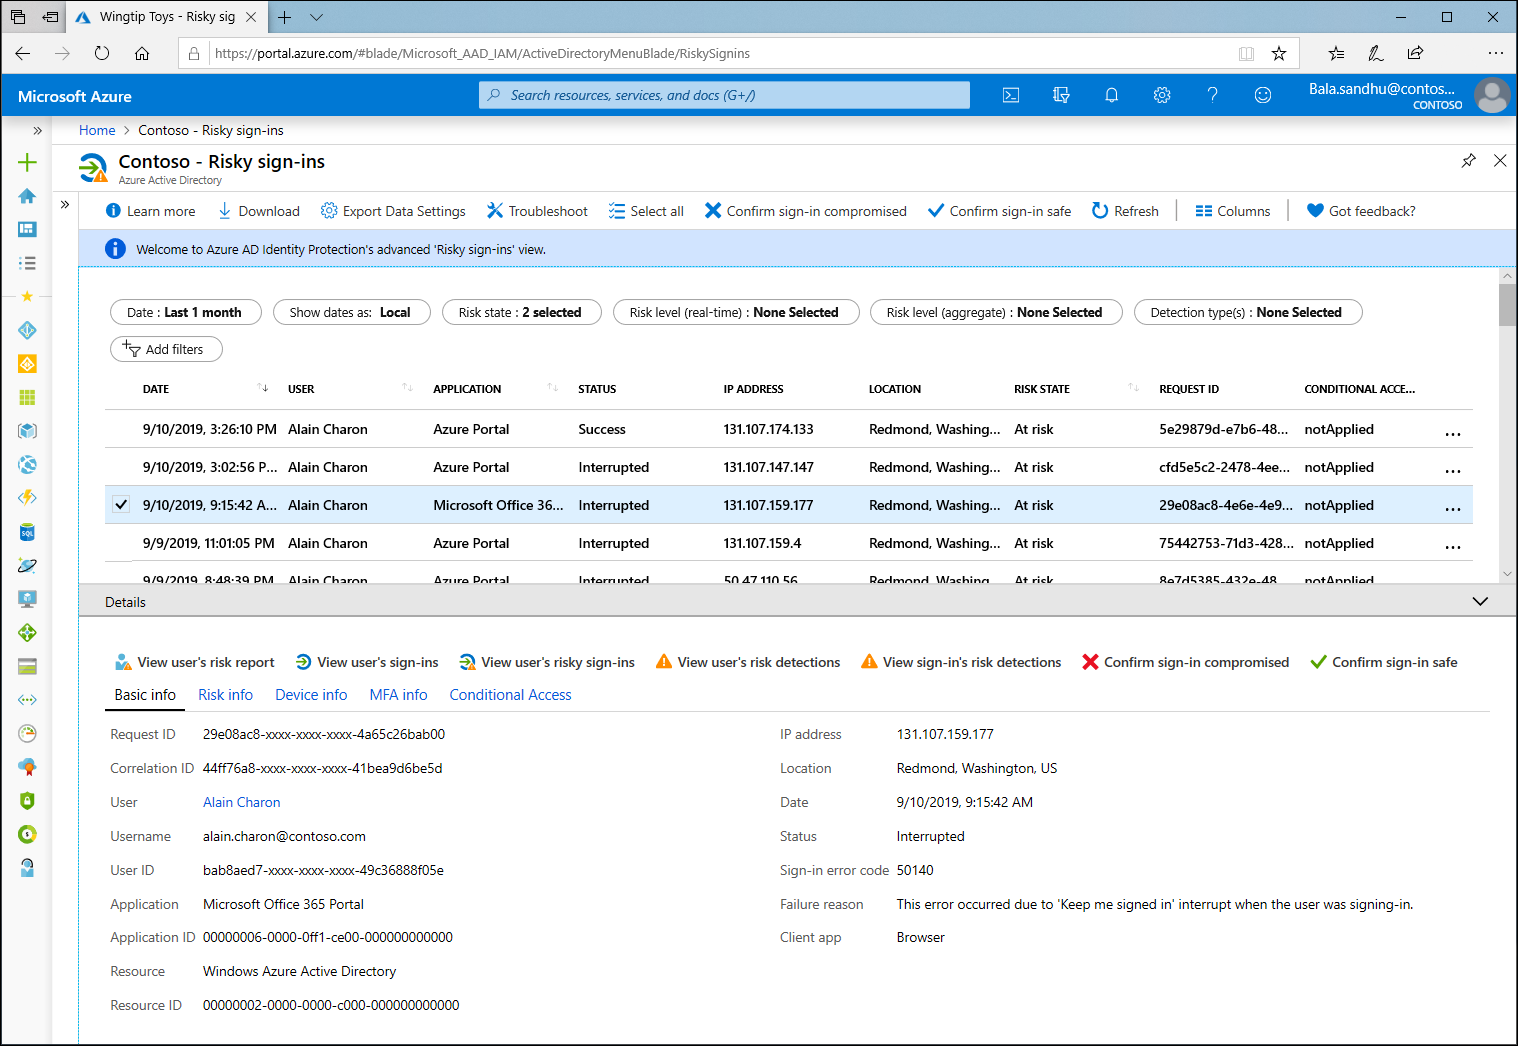
\includegraphics[width=0.8\textwidth]{identity-protection-risky-sign-ins-report.png}
\caption{Identify protection risky sign-ins report}
\end{figure}

\textbf{Remediation}
\begin{enumerate}
\item Technical tools
	\begin{enumerate}
	\item Azure Multi-Factor Authentication
	\item Reset their password using self-service password reset
	\item Blocking until an administrator takes action
	\end{enumerate}
\item Policies
	\begin{enumerate}
	\item MFA registration policy. \textit{Can help organizations roll out MFA using a Conditional Access policy requiring registration at sign-in.}
	\item Sign-in risk policy. \textit{Analyzes signals from each sign-in, both real-time and offline, and calculates a risk score based on the probability that the sign-in wasn't performed by the user. If risk is detected, users can perform multi-factor authentication to self-remediate and close the risky sign-in event to prevent unnecessary noise.}
	\item User risk policy. \textit{Calculate what it believes is normal for a user's behaviour and use that to base decisions for their risk. If risk is detected, users can perform self-service password reset to self-remediate and close the user risk event to prevent unnecessary noise.}
	\end{enumerate}
\end{enumerate}

\textbf{License requirements} \\
\begin{tabular}{l p{6cm} c c c}

 &  & Premium P2 & Premium P1 & Basic/Free \\
Risk policies & User risk policy & \cmark & \xmark & \xmark \\
Risk policies & Sign-in risk policy & \cmark & \xmark & \xmark \\
Security reports & Overview & \cmark & \xmark & \xmark \\
Security reports & Risky users & \cmark & Limited & Limited \\
Security reports & Risky sign-ins & \cmark & Limited & Limited \\
Security reports & Risk detections & \cmark & Limited & \xmark \\
Notifications & Users at risk detected alerts & \cmark & \xmark & \xmark \\
Notifications & Weekly digest & \cmark & \xmark & \xmark \\
	& MFA registration policy & \cmark & \xmark & \xmark \\
\end{tabular}

\textbf{Users role with Identity Protection access}
\begin{enumerate}
\item Security Reader
\item Security Operator
\item Security Administrator
\item Global Reader
\item Global Administrator
\end{enumerate}

\subsubsection{Azure AD Connect}
\textbf{Wizards} 
\begin{itemize}
\item Express. Requires high level of privileges and does not require creating users or configuring permissions. Requires two accounts a) AD DS Enterprise Administrator and b) Azure AD Global Administrator.

\item Custom. It is used in all cases where the express installation option does not satisfy your deployment or topology.
\end{itemize}

\textbf{Accounts} 
\begin{itemize}
\item Synchronisation
	\begin{itemize}
	\item AD DS Connector account: \\ Used to read/write information to Windows Server Active Directory.
	\item ADSync service account: \\ Used to run the synchronization service and access the SQL database.
	\item Azure AD Connector account: \\ Used to write information to Azure AD.
	\end{itemize}
\item Installation
	\begin{itemize}
	\item Local Administrator account: \\ The administrator who is installing Azure AD Connect and who has local Administrator permissions on the machine.
	\item AD DS Enterprise Administrator account: \\ Optionally used to create the "AD DS Connector account" above.
	\item Azure AD Global Administrator account: \\ Used to create the Azure AD Connector account and configure Azure AD. \\ After installation this account should be changed from Global Administrator role to the \textit{Directory Synchronization Accounts} role.
	\item SQL SA account (optional): \\ Used to create the ADSync database when using the full version of SQL Server. This account could be the same account as the Enterprise Administrator. 
	\end{itemize}
\end{itemize}
\begin{figure}[!h]
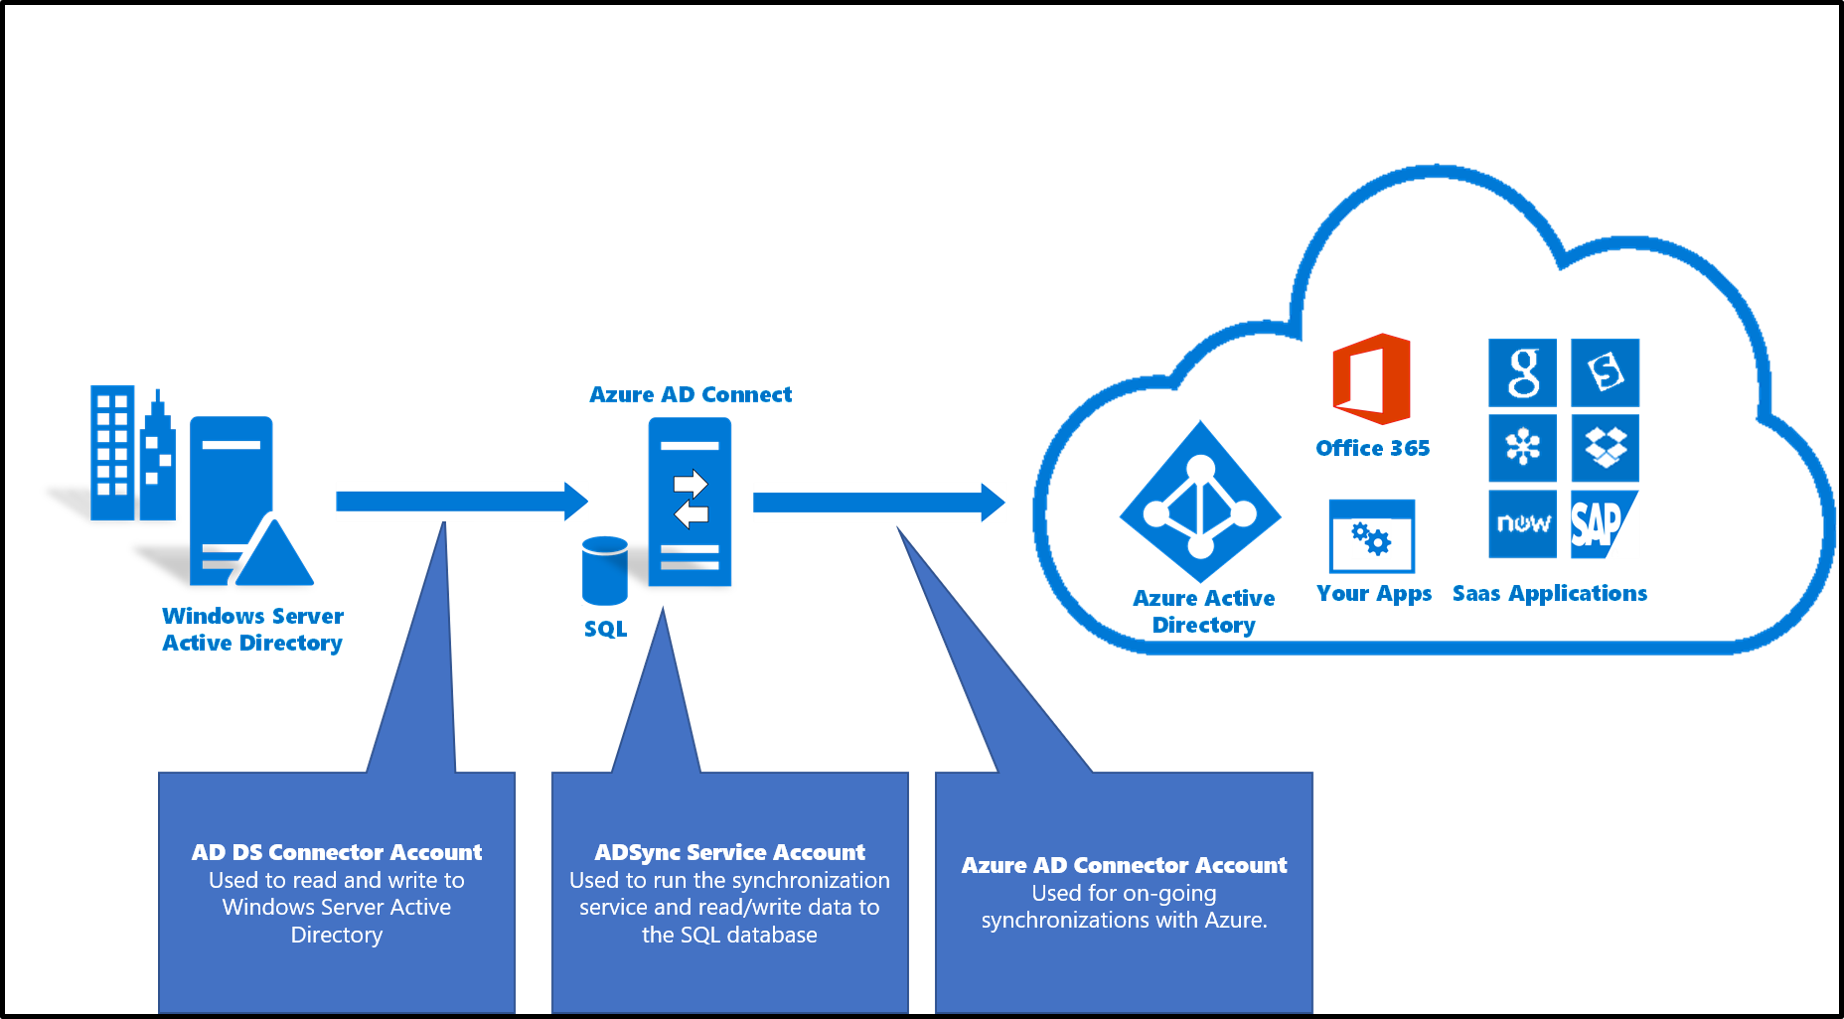
\includegraphics[width=1\textwidth]{azure-ad-connect-account.png}
\caption{Accounts used for Azure AD Connect}
\label{fig:azure-connect-accounts}
\end{figure}

\textbf{Components}
\begin{itemize}
\item SQL Server 2012 Express, LocalDB instance
\item User sign-in scheme
	\begin{itemize}
	\item Password Hash Sync. \textit{The users passwords are synchronized to Azure AD as a password hash and authentication occurs in the cloud.}
	\item Pass-through Authentication. \textit{The users password is passed through to the on-premises Active Directory domain controller to be validated.}
	\item Federation with AD FS. \textit{The users are redirected to their on-premises AD FS instance to sign in and authentication occurs on-premises.}
	\item Federation with PingFederate. \textit{ The users are redirected to their on-premises PingFederate instance to sign in and authentication occurs on-premises.}
	\item Do not configure. \textit{No user sign-in feature is installed and configured. Choose this option if you already have a 3rd party federation server or another existing solution in place.}
	\item [Option] Enable Single Sign on. \textit{Provides a single sign on experience for desktop users on the corporate network. For Hash or Pass-through.}
	\end{itemize}
\end{itemize}

% Configure Microsoft Azure AD Privileged Identity Management %
% This section contains notes on "Configure Microsoft Azure AD Privileged Identity Management" relevant subjects %
\subsubsection{Privileged identity management}
Privileged identity management seeks to accomplish:
\begin{itemize}
\item Integrated access reviews 
\item Manage risk : least privilege access
	\begin{itemize}	
	\item Just-in-time access
	\item Request approval workflows
	\end{itemize}
\item Address compliance and governance
\item Prevention of malicious activities in real time
\end{itemize}

\textbf{Setup}
\begin{enumerate}
\item Sign in. \textit{As global administrator.}
\item Navigate to PIM service. \textit{Click All services and find the Azure AD Privileged Identity Management service.}
\item Setup MFA for account. \textit{If not already done.}
\item Consent to PIM. \textit{Automatically assigned the Security Administrator and Privileged Role Administrator roles.}
\item Verify identify. \textit{With MFA.}
\end{enumerate}

\textbf{Deployment} 
\begin{enumerate}
\item Identify stakeholders
\item Enable Privileged Identity Management
\item Enforce principle of least privilege
	\begin{enumerate}
	\item Understand the granularity of the roles
	\item List who has privileged roles in your organization
	\item Reduce the amount of Global Administrators. \textit{Consider automating with acess review}.
	\item Reduce other administrators. \textit{Consider automating with acess review}.
	\end{enumerate}
\item Decide which role assignments should be protected by Privileged Identity Management
	\begin{enumerate}
	\item Should be atleast Global Administrators and Security Administrators
	\item All guest users
	\item Owner roles and User Access Administrator roles of all subscriptions/resources
	\end{enumerate}
\item Decide which role assignments should be permanent or eligible
	\begin{enumerate}
	\item Two break-glass emergency access accounts
	\end{enumerate}
\item Draft your Privileged Identity Management settings
\end{enumerate}
\begin{enumerate}
\item Use Privileged Identity Management alerts to safeguard your privileged access
\item Set up recurring access reviews to regularly audit your organization’s privileged identities
	\begin{enumerate}
	\item Quarterly access reviews for all your Azure AD and Azure resource roles
	\item Secondary email address for all accounts with privileged role assignments that are not linked to a regularly checked email address
	\end{enumerate}
\item Get the most out of your audit log to improve security and compliance
	\begin{enumerate}
	\item Read all audit events on a weekly basis and export your audit events on a monthly basis
	\item Use Azure log monitoring to archive audit events in an Azure storage account for the need of security and compliance
	\end{enumerate}
\end{enumerate}

\textbf{Features} \\
\begin{tabular}{p{3cm} p{12cm}}
\textbf{Tasks} \\
My roles & List of eligible\footnote{A role assignment that requires a user to perform one or more actions to use the role. If a user has been made eligible for a role, that means they can activate the role when they need to perform privileged tasks. These can be viewed and activated here.} and active roles assigned to you. \\
My requests & Pending requests to activate eligible role assignments. \\
Approve requests & Requests to activate eligible roles, that you are designated to approve. \\
Review access & Active access reviews you are assigned to complete, whether you're reviewing access for yourself or someone else. \\
\textbf{Manage} \\
Azure AD roles & Dashboard and settings to manage Azure AD role assignments. \newline \textit{Only for privileged role administrators.} \\
Azure resources & Dashboard and settings to manage Azure resource role assignments. \newline \textit{Only for privileged role administrators.} \\
\end{tabular}

\textbf{Restrictions} \\
Privileged Identity Management does not allow the management for all roles. Specifically some classic subscription administrator roles and some Exchange and Sharepoint roles.
\begin{itemize}
\item Account Administrator
\item Service Administrator
\item Co-Administrator
\item Exchange Online roles 
\item SharePoint Online roles
\end{itemize}
Exchange Administrator and SharePoint Administrator are available, but can experience delays. 

\begin{figure}[!h]
\centering
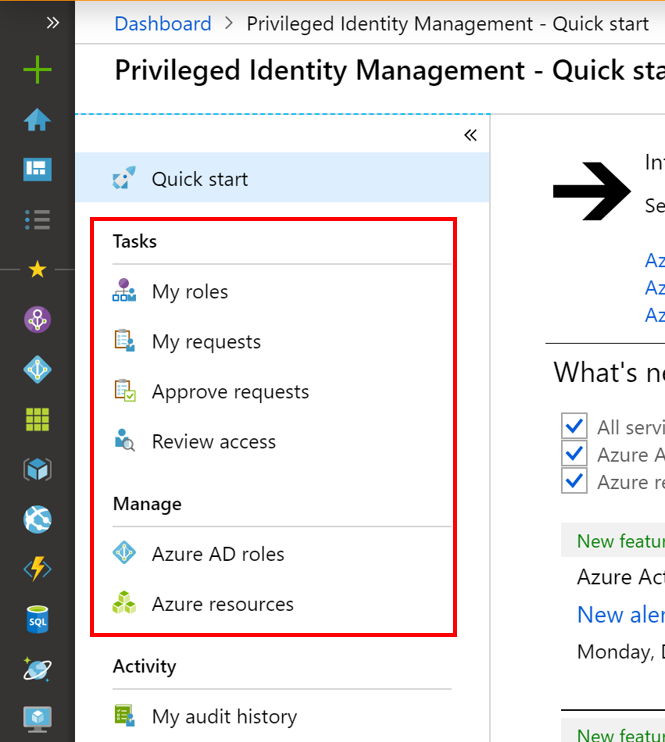
\includegraphics[width=0.5\textwidth]{pim-quickstart-tasks.png}
\caption{Privileged Identity Management - Quick start}
\label{fig:azure-connect-accounts}
\end{figure}

Depending on the Privileged Identity Management settings configured for the role, the user must complete certain steps (such as performing multi-factor authentication, getting approval, or specifying a reason.)

\textbf{License requirements}
\begin{itemize}
\item Azure AD Premium P2
\item Enterprise Mobility + Security (EMS) E5
\item Microsoft 365 M5
\end{itemize}

\textbf{User roles with Privileged Identity Management access}
Each administrator or user who interacts with or receives a benefit from Privileged Identity Management must have a license. Examples include:
\begin{itemize}
\item Administrators
	\begin{itemize}
	\item with Azure AD roles managed using PIM
	\item Azure resource roles managed using PIM
	\item assigned to the Privileged Role Administrator role
	\end{itemize}
\item Users
	\begin{itemize}
	\item assigned as eligible to Azure AD roles managed using PIM
	\item able to approve/reject requests in PIM
	\item assigned to an Azure resource role with just-in-time or direct (time-based) assignments
	\item assigned to an access review
	\item who perform access reviews
	\end{itemize}
\end{itemize}

\textbf{Trivia and quirks} 
\begin{enumerate}
\item First person to use Privileged Identity Management in your directory, is automatically assigned the Security Administrator and Privileged Role Administrator roles
\item Only \textit{organizational} accounts, with Global Administrator role, can enable Privileged Identity Management for a directory
\end{enumerate}

\subsubsection{Access review}


% Configure Microsoft Azure tenant security %
\subsubsection{Azure Tenants}
\textbf{Transferring subscriptions} \\
It is possible to transfer a subscription to another tenant, this will remove all role-based access control (RBAC) assignments to manage resources in the original subscription. It is also possible to transfer just the billing ownership of an account, without moving the subscription to the new accounts tenant - this is done by unchecking the box for Subscription Azure AD.

\textbf{External developer account} \\
It is possible to enable access to the developer portal for users from Azure Active Directory (Azure AD). This is intended to provide access for external developers and this feature is available in the Premium, Standard and Developer tiers of API Management.



\clearpage
%%% Notes for Implement platform protection %%%
\subsection{Implement platform protection}

% Implement network security
\subsubsection{Implement network security}

\textbf{Azure Virtual Network} \\
Design best practices:
\begin{enumerate}
\item Minimise conflicts. \textit{Ensure non-overlapping address spaces. The VNet address space (CIDR block) should not overlap with your organization's other network ranges.}
\item Keep a reserve space. \textit{Reserve some of the address space of the VNet.}
\item Minimise management overhead. \textit{Create a few large VNets, rather than multiple small VNets.}
\item Secure it. \textit{Secure your VNet using Network Security Groups (NSGs)}.
\end{enumerate}

Communication: \\
All resources in a VNet can communicate outbound to the internet, by default. You can communicate inbound to a resource by assigning a public IP address or a public Load Balancer. When using only an internal Standard Load Balancer, outbound connectivity is not available until you define how you want outbound connections to work with an instance-level public IP or a public Load Balancer.

The communication options of Azure resources are:
\begin{itemize}
\item Virtual network: \textit{Deploy VMs, and other Azure resources to a virtual network, such as Azure App Service Environments, the Azure Kubernetes Service (AKS), or Azure Virtual Machine Scale Sets.}
\item Through a virtual network service endpoint: \textit{Extend your virtual network private address space and the identity of your virtual network to Azure service resources, such as Azure Storage accounts and Azure SQL databases, over a direct connection. Service endpoints allow you to secure your critical Azure service resources to only a virtual network.}
\item VNet Peering: \textit{Connect virtual networks to each other, enabling resources in either virtual network to communicate with each other, using virtual network peering. The virtual networks you connect can be in the same, or different, Azure regions.}
\end{itemize}

The communication options for on-premise resources are:
\begin{itemize}
\item Point-to-site virtual private network (VPN): \textit{Established between a virtual network and a single computer in your network. Each computer must configure an individual connection. Intended for developers, as it requires few adjustments to existing network. The communication is encrypted.}
\item Site-to-site VPN: \textit{Established between on-premises VPN device and an Azure VPN Gateway in a virtual network. This connection type enables any on-premises resource that you authorize to access a virtual network. The communication is encrypted.}
<<<<<<< HEAD
\item Azure ExpressRoute: \textit{Established between your network and Azure, through an ExpressRoute partner. This connection is private. Traffic does not go over the internet.}
=======
\item Azure ExpressRoute: \textit{Established between your network and Azure, through an ExpressRoute partner. This connection is private. Traffic does not go over the internet.} This is not encrypted by default.
>>>>>>> 728182d4551be8fca7f552b0874ef019cc3f6d12
\end{itemize}

You can filter network traffic between subnets using either or both of the following options:
\begin{itemize}
\item Security groups: \textit{Network security groups and application security groups can contain multiple inbound and outbound security rules that enable you to filter traffic to and from resources by source and destination IP address, port, and protocol.}
\item Network virtual appliances:\textit{A network virtual appliance is a VM that performs a network function, such as a firewall, WAN optimization, or other network function.}
\end{itemize}

Azure routes traffic between subnets, connected virtual networks, on-premises networks, and the Internet, by default. You can implement either or both of the following options to override the default routes Azure creates:
\begin{itemize}
\item Route tables: \textit{Custom route tables with routes that control where traffic is routed to for each subnet.}
\item Border gateway protocol (BGP) routes: \textit{Connect the virtual network to the on-premises network using an Azure VPN Gateway or ExpressRoute connection, you can propagate your on-premises BGP routes to your virtual networks. }
\end{itemize}

\textbf{Network Security Groups} \\
Security rules in network security groups enable you to filter the type of network traffic that can flow in and out of virtual network subnets and network interfaces.

A network security group (NSG) contains a list of security rules that allow or deny network traffic to resources connected to Azure Virtual Networks (VNet). NSGs can be associated to subnets, individual VMs (classic), or individual network interfaces (NIC) attached to VMs (Resource Manager).  When an NSG is associated to a subnet, the rules apply to all resources connected to the subnet. Traffic can further be restricted by also associating an NSG to a VM or NIC.

\begin{figure}[!h]
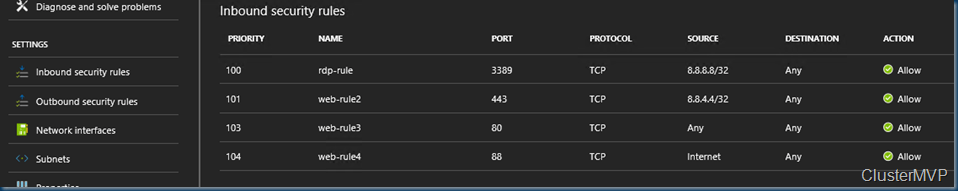
\includegraphics[width=1\textwidth]{platform-network-rules.png}
\caption{List of inbound security rules}
<<<<<<< HEAD
\end{figure}


\textbf{Application Security Groups} \\
Feature for security micro-segmentation for your virtual networks in Azure.
\begin{figure}[!h]
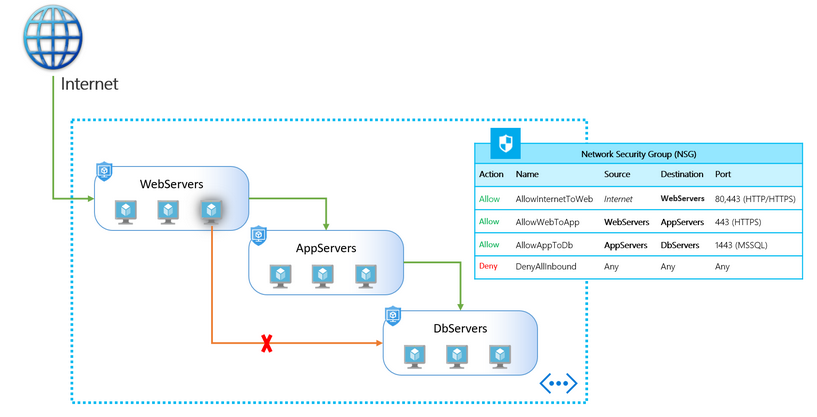
\includegraphics[width=1\textwidth]{platform-network-application-security-groups.png}
\caption{Application Security Groups (ASG) in all Azure regions}
\end{figure}

\underline{Network segmentation.} Centralized on applications, instead of explicit IP addresses. Implementing granular security traffic controls improves isolation of workloads and protects them individually. 

Filtering traffic based on applications patterns
\begin{itemize}
\item Define your application groups
\item Define a single collection of rules using ASGs and Network Security Groups (NSG)
\item Scale at your own pace. When you deploy VMs, make them members of the appropriate ASGs. \textit{Implement a zero-trust model, limiting access to the application flows that are explicitly permitted.}
\end{itemize}

\textbf{Firewall} \\
Outbound network access controls:
\begin{itemize}
\item Application rules that define fully qualified domain names (FQDNs) that can be accessed from a subnet.
\item Network rules that define source address, protocol, destination port, and destination address.
\end{itemize}

\subsubsection{Security management}
For more secure management and operations, you can minimize a client’s attack surface by reducing the number of possible entry points. This can be done through security principles: “separation of duties” and “segregation of environments.”

\begin{itemize}
\item Isolate sensitive functions \textit{from one another to decrease the likelihood that a mistake at one level leads to a breach in another. I.e. do not perform tasks such as browsing or email on secured workstations.}
\item Reduce the system’s attack surface by removing unnecessary software \textit{i.e. email client and productivity applications.}
\item Secure management workstations. \textit{Client systems that have administrator access to infrastructure components should be subjected to the strictest possible policy to reduce security risks.}
	\begin{itemize}
	\item Security policies > Group Policy > Deny open Internet access
	\item Use Internet Protocol security (IPsec) VPNs if direct access is needed
	\item Separate management and development Active Directory domains
	\item Isolate and filter management workstation network traffic
	\item Antimalware software
	\item Multi-factor authentication 
	\end{itemize}
\end{itemize}

\textbf{Security mechanisms}\\
Azure provides security mechanisms to aid administrators who manage Azure cloud services and virtual machines. These mechanisms include:

\begin{itemize}
\item Authentication and role-based access control.
\item Monitoring, logging, and auditing.
\item Certificates and encrypted communications.
\item A web management portal.
\item Network packet filtering.
\end{itemize}

\textbf{Hardened workstation}
\begin{itemize}
\item Active scanning and patching.
\item Limited functionality.
\item Network hardening. \textit{Use Windows Firewall rules to allow only valid IP addresses, ports, and URLs related to Azure management. Ensure that inbound remote connections to the workstation are also blocked.}
\item Execution restriction. \textit{Allow only a set of predefined executable files that are needed for management to run (referred to as “default-deny”).}
\item Least privilege. \textit{Management workstation users should not have any administrative privileges on the local machine itself. }
\end{itemize}
You can enforce all this by using Group Policy Objects (GPOs) in Active Directory Domain Services (AD DS) and applying them through your (local) management domain to all management accounts.

\begin{itemize}
\item IE hardening. \textit{Review your client policies and enforce running in protected mode, disabling add-ons, disabling file downloads, and using Microsoft SmartScreen filtering. Ensure that security warnings are displayed. Take advantage of Internet zones and create a list of trusted sites for which you have configured reasonable hardening. Block all other sites and in-browser code, such as ActiveX and Java.}
\item Standard user. \textit{Running as a standard user brings a number of benefits, the biggest of which is that stealing administrator credentials via malware becomes more difficult. In addition, a standard user account does not have elevated privileges on the root operating system, and many configuration options and APIs are locked out by default.}
\item AppLocker. \textit{Use AppLocker to restrict the programs and scripts that users can run. You can run AppLocker in audit or enforcement mode. By default, AppLocker has an allow rule that enables users who have an admin token to run all code on the client.}
\item Code signing. \textit{Code signing all tools and scripts used by administrators provides a manageable mechanism for deploying application lockdown policies. Hashes do not scale with rapid changes to the code, and file paths do not provide a high level of security. You should combine AppLocker rules with a PowerShell execution policy that only allows specific signed code and scripts to be executed.}
\item Group Policy. \textit{Create a global administrative policy that is applied to any domain workstation that is used for management (and block access from all others), and to user accounts authenticated on those workstations.}
\item Security-enhanced provisioning. \textit{Safeguard your baseline hardened workstation image to help protect against tampering. Use security measures like encryption and isolation to store images, virtual machines, and scripts, and restrict access (consider using an auditable check-in/check-out process).}
\item Patching. 
\item Encryption. \textit{Make sure that management workstations have a Trusted Platform Module}
\item Governance. Use \textit{AD DS GPOs to control all the administrators’ Windows interfaces, such as file sharing. Include management workstations in auditing, monitoring, and logging processes. Track all administrator and developer access and usage.}
\end{itemize}

\textbf{Best practices} \\
\begin{tabular}{p{7.3cm} p{7.3cm}}
\textbf{Do} & \textbf{Don't} \\
\hline 
Maintain confidentiality by delivering account names and passwords directly, perform a remote installation of client/server certificates (via an encrypted session), download from a protected network share, or distribute by hand via removable media. & Don't email credentials for administrator access or other secrets (for example, SSL or management certificates) \\
\hline 
Proactively manage certificate life cycles. &  \\
\hline 
Establish security management principles and system hardening policies. Apply them to your development environments. & Don't store account passwords unencrypted or un-hashed. \\
\hline 
Use Enhanced Mitigation Experience Toolkit 5.5 certificate pinning rules to ensure proper access to Azure SSL/TLS sites. &  \\
\hline 
Create a dedicated Microsoft account to manage your Azure subscription & Don't share accounts and passwords between administrators, or reuse passwords across multiple user accounts or services, particularly those for social media or other non-administrative activities. \\
\hline
Configuration files and profiles should be installed from a trusted source. & Don't email configuration files. \\
\hline
Enforce strong password policies, expiration cycles (changeon-first-use), console timeouts, and automatic account lockouts. Use a client password management system with multi-factor authentication for password vault access. & Don't use weak or simple logon passwords. \\
\hline
Lock down Azure ports and IP addresses to restrict management access. & Don't expose management ports to the Internet. \\
\hline
Use firewalls, VPNs, and NAP for all management connections.
\end{tabular}

\clearpage
\textbf{Azure Storage firewalls} \\
Azure Storage provides a layered security model. This model enables you to secure and control the level of access to your storage accounts that your applications and enterprise environments demand, based on the type and subset of networks used. When network rules are configured, only applications requesting data over the specified set of networks can access a storage account. You can limit access to your storage account to requests originating from specified IP addresses, IP ranges or from a list of subnets in an Azure Virtual Network (VNet).

An application that accesses a storage account when network rules are in effect still requires proper authorization for the request. Authorization is supported with Azure Active Directory (Azure AD) credentials for blobs and queues, with a valid account access key, or with an SAS token.

Turning on firewall rules for your storage account blocks incoming requests for data by default, unless the requests originate from a service operating within an Azure Virtual Network (VNet) or from allowed public IP addresses. Requests that are blocked include those from other Azure services, from the Azure portal, from logging and metrics services, and so on.

You can grant access to Azure services that operate from within a VNet by allowing traffic from the subnet hosting the service instance. You can also enable a limited number of scenarios through the Exceptions mechanism.

\begin{tabular}{c c p{6cm}}

\end{tabular}
=======
\end{figure}
>>>>>>> 728182d4551be8fca7f552b0874ef019cc3f6d12

\section{Quiz}
\subsection{Manage identity and access}
As an enterprise or software-as-a-service (SaaS) developer you which to build an application which allows users to sign in using their Personal Microsoft accounts. Which Microsoft Identity platform library provides authentication tools for Personal Microsoft accounts?
\begin{todolist}
\item Microsoft Authentication Library (MSAL)
\item Azure AD Authentication Library (ADAL)
\item .NET DotNetOpenAuth (OAuth)
\item Microsoft Active Directory Library (MADL)
\end{todolist}
\begin{center}\rule{6cm}{0.4pt}\end{center}
An application which allows users to update their contact information, is created utilising the delegated permission scheme. Can the current user signed in, Bob from HR, update the contact information of his colleague Alice, using the application? \textit{The application has the User.ReadWrite.All delegated permission in Microsoft Graph.}
\begin{todolist}
\item Yes. The effective permissions granted by the application allows signed-in user the ability to update all users.
\item No. The effective permissions granted by the application does not allow signed-in user the ability to update all users.
\end{todolist}
\begin{center}\rule{6cm}{0.4pt}\end{center}
As part of a merger is is necessary to transfer the billing ownership of several user accounts. Which of the these account types can have their billing ownership transferred.
\begin{todolist}
\item Azure in Open (AIO)
\item Visual Studio Enterprise (MPN) subscribers
\item Visual Studio Professional
\item Microsoft Partner Network
\item Free Trial
\item Pay-As-You-Go
\end{todolist}
\begin{center}\rule{6cm}{0.4pt}\end{center}

\vspace{1cm}
\textcolor{red}{\textit{Create additional questions from \href{https://docs.microsoft.com/en-us/azure/active-directory/develop/v2-permissions-and-consent\#using-the-admin-consent-endpoint}{https://docs.microsoft.com/en-us/azure/active-directory/develop/v2-permissions-and-consent\#using-the-admin-consent-endpoint}}}
\section{Quiz (with answers)}
\subsection{Manage identity and access}
As an enterprise or software-as-a-service (SaaS) developer you which to build an application which allows users to sign in using their Personal Microsoft accounts. Which Microsoft Identity platform library provides authentication tools for Personal Microsoft accounts?
\begin{todolist}
\item[\correct] Microsoft Authentication Library (MSAL)
\item[\incorrect] Azure AD Authentication Library (ADAL)
\item[\incorrect] .NET DotNetOpenAuth (OAuth)
\item[\incorrect] Microsoft Active Directory Library (MADL)
\end{todolist}
\end{appendices}

\end{document}